\documentclass[11pt]{article}

% include packages
\usepackage{lipsum}
\usepackage[margin=1 in,includefoot]{geometry}
\usepackage[utf8]{inputenc}
\usepackage{hyperref}

%%%%%Graphics
\usepackage{graphicx}
\usepackage{float}

%%%%Biblio


%%%%%%%% Header and footer
\usepackage{fancyhdr}
\pagestyle{fancy}
\fancyhead{}
\fancyfoot{}
\fancyfoot[R]{\thepage}
\renewcommand{\headrulewidth}{0pt}
\renewcommand{\footrulewidth}{1pt}

% deal with hyper link of table of contents and references
\hypersetup{
    colorlinks=true, %set true if you want colored links
    linktoc=all,     %set to all if you want both sections and subsections linked
    linkcolor=black,  %choose some color if you want links to stand out
}
%%%%%%%%%%%%%%%%%%%%%

% edit start
\begin{document}

% title
\begin{titlepage}
\title{
	{\large People in Ecosystems/Watershed Integration (PEWI)}\\
	{\huge {Advanced Level Glossary Notes\\}}
	% including logo image
	\begin{figure}[H]
	\centering
	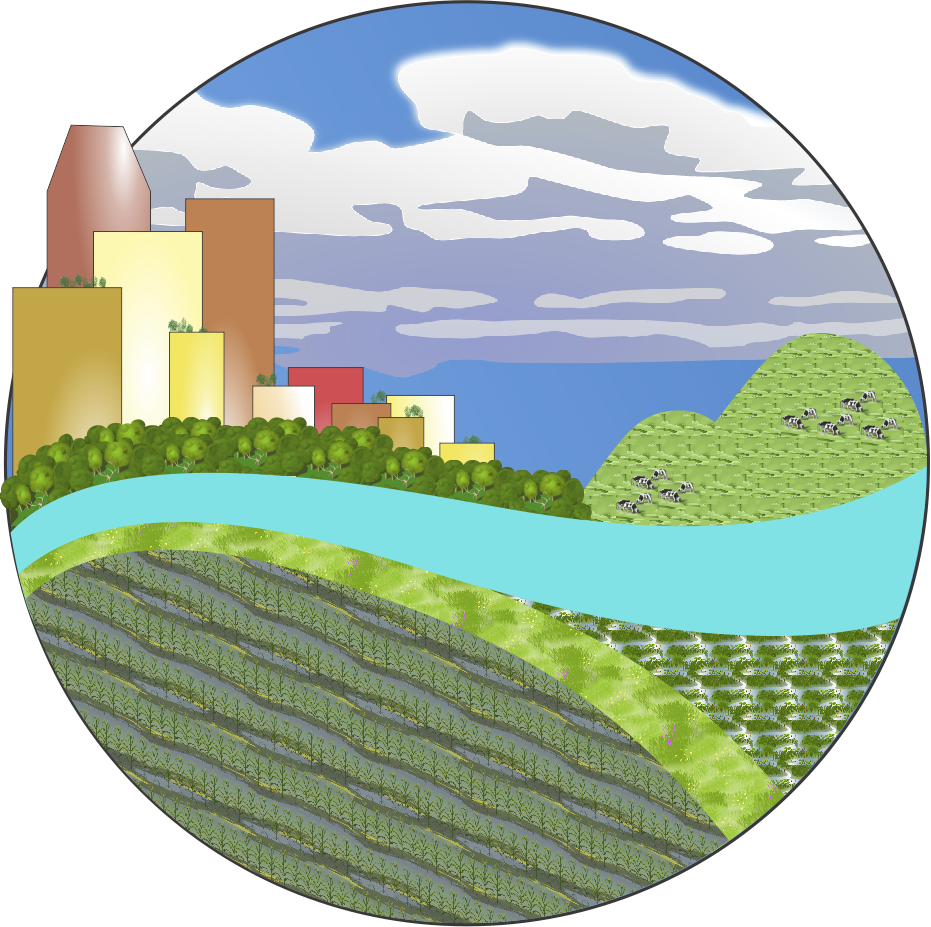
\includegraphics[height=3 in]{../imgs/updatedPewiLogo.png}
	\end{figure}
}
\author{ \centering
	\begin{tabular}{rl}
   \quad \textbf{PEWI Team}\\
  \\
  \centering
  \textbf{Project Leads: } \\
  Lisa Sculte Moore & Robert Valek\\
  \\
  \centering
  \textbf{Team Members: } \\
  Uma Abu & Han-Shu Chang\\
  Nancy Grudens-Schuck & Elizabeth Li\\
  Lisa Schulte Moore & Alexander Schulz \\
  Mehul Shinde & John Tyndall \\
  Robert Valek & John VanDyk \\
\end{tabular}
}
\date {\today} % date
\maketitle
\thispagestyle{empty} % no page number on cover
\end{titlepage}

\newpage
% stuff before table of contents
\pagenumbering{roman}
\section*{Summary}
\addcontentsline{toc}{section}{\numberline{}Summary}
This is the document of index. This document includes all descriptions for the general tab.
\cleardoublepage

\section*{Acknowledgements}
\addcontentsline{toc}{section}{\numberline{}Acknowledgements}
Funding from The McKnight Foundation , US Forest Service Northern Research Station , Iowa State University Department of Agronomy , Leopold Center for Sustainable Agriculture, and USDA McIntire-Stennis Program have supported development of PEWI . We thank Assata Caldwell , Cindy Cambardella , Carrie Chennault , Justin Choe , Diane Debinski , Ranae Dietzel , Stephanie Enloe , Ryan Frahm , Nancy Grudens-Schuck , Emily Heaton , Matt Helmers , Noah Hagen , Jake Hill , Michael Hofmockel , Tom Isenhart , Charlie Labuzzetta , Matt Liebman , Devan McGranahan , Elise Miller , Larysa Nadolny , Laura Roy , Nancy Shyrock , John Van Dyk , and the Natural Capital Project for contribution to PEWI’s development and review.
\cleardoublepage


%%%%%Table of content starts here
\tableofcontents
\thispagestyle{empty} % no page number on table of contents page
\cleardoublepage % no other contents on table of contents page

%%% to start page numbers from 1
\pagenumbering{arabic}
\setcounter{page}{1}

% === main contents ===

% Land Use section
\section{Land Use}\label{sec:landuse}
Upland grid cells, those not containing part of the river, are 10 acres (4 hectares) in area. Grid cells along the river decrease in area to account for the percent of the grid cell underwater. Land use for a particular land cover is calculated by the sum of the area of each grid cell using that land cover. To find percent land use, this sum is divided by the total area of the watershed and multiplied by 100.

% sub section
\subsection{Conventional Corn}

Corn performs best on gentle terrain with high drainage and low flooding probability. The conventional corn land cover in PEWI assumes conventional tillage and no use of cover crops, terraces, contours, grassed waterways, or stream buffers.

Strategic placement can maximize your per-unit yield: Muscatine 119, Tama 120B, Nicollet 55, and Clarion 138B soils are highly productive for annual crops in general, while Buckney 1636 and Gara-Armstrong 993E2 soils are unproductive.

With a conventional corn-dominated land cover, yield, erosion control, and nitrate, phosphorus, and sediment retention vary significantly under different precipitation scenarios.

To improve ecosystem scores in extreme precipitation conditions, try switching from conventional to conservation crops.

Conventional crops also do not provide points in the wildlife habitat or carbon sequestration categories. To improve habitat scores, try adding some perennial or native habitat. To improve carbon sequestration scores, try adding some woody land covers or wetlands.


\subsection{Conventional Soy}

Soybeans perform best on gentle terrain with high drainage and low flooding probability. The conventional soybean land cover in PEWI assumes conventional tillage and no use of cover crops, terraces, contours, grassed waterways, or stream buffers.
Strategic placement can maximize your per-unit yield: Muscatine 119, Tama 120B, Nicollet 55, and Clarion 138B soils are highly productive for annual crops in general, while Buckney 1636 and Gara-Armstrong 993E2 soils are unproductive.

With a conventional soy-dominated land cover, yield, erosion control, and nitrate, phosphorus, and sediment retention vary significantly under different precipitation scenarios.

To improve ecosystem scores in extreme precipitation conditions, try switching from conventional to conservation crops.

Conventional crops also do not provide points in the wildlife habitat or carbon sequestration categories. To improve habitat scores, try adding some perennial or native habitat. To improve carbon sequestration scores, try adding some woody land covers or wetlands.

\subsection{Conservation Corn}

Corn performs best on gentle terrain with high drainage and low flooding probability.

Strategic placement can maximize your per-unit yield: Muscatine 119, Tama 120B, Nicollet 55, and Clarion 138B soils are highly productive for annual crops in general, while Buckney 1636 and Gara-Armstrong 993E2 soils are unproductive.

Conservation corn base yield is equivalent to that of conventional corn.

One hundred percent conservation corn cover gives sediment retention scores above 90, and phosphorus retention and erosion control scores above 85 in all precipitation scenarios. Nitrate retention varies substantially under different precipitation scenarios. To improve nitrate retention scores in extreme precipitation conditions, try switching to perennial land uses.

Conservation crops provide minimal carbon sequestration and moderate habitat points. To improve carbon sequestration scores, try adding some woody land covers or wetlands. To improve habitat scores, try adding some native vegetation.

\subsection{Conservation Soy}

Soybeans perform best on gentle terrain with high drainage and low flooding probability.

Strategic placement can maximize your per-unit yield: Muscatine 119, Tama 120B, Nicollet 55, and Clarion 138B soils are highly productive for annual crops in general, while Buckney 1636 and Gara-Armstrong 993E2 soils are unproductive.

Conservation soybean base yield is equivalent to that of conventional soybean.

One hundred percent conservation soybean cover gives sediment retention scores above 90, and phosphorus retention and erosion control scores above 80 in all precipitation scenarios. Nitrate retention varies substantially under different precipitation scenarios. To improve nitrate retention scores in extreme precipitation conditions, try switching to perennial crops.

Conservation crops provide minimal points in carbon sequestration, and moderate habitat points. To improve carbon sequestration scores, try adding some woody land covers or wetlands. To improve habitat scores, try adding some native vegetation.

\subsection{Alfalfa}

Alfalfa performs best on soils with excessive to moderate drainage.

Strategic placement can maximize your per-unit yield: Tama 120B, Muscatine 119, Tama 120C2, Nicollet 55, Nodaway 220, and Clarion 138B soils are highly productive for alfalfa and grass hay, while Buckney 1636, Okoboji 90, and Gara-Armstrong 993E2 soils are approximately half as productive.

Yield varies only slightly in extreme precipitation scenarios.

One hundred percent alfalfa land cover gives the maximum score in nitrate retention, erosion control and sediment retention scores above 90, and phosphorus retention above 80 in all precipitation scenarios. Phosphorus contribution is decreased for areas with an elevation grade of less than 9%.

Alfalfa does not provide points in the habitat categories and provides only minimal carbon sequestration benefit. To improve habitat scores, try switching to grass hay or adding some native vegetation or stream buffers. To improve carbon sequestration scores, try adding some woody land covers or wetlands.

\subsection{Mixed Fruit and Vegetables}

Mixed fruit and vegetables perform best on fine sandy loam, silt loam, or loam.

Strategic placement can maximize your per-unit yield: Buckney 1636, Downs 162D2, Nodaway 220, Ackmore-Colo 5B, Muscatine 119, and Gara-Armstrong 993E2 soils are highly productive for mixed fruit and vegetables, while all other soils are less than half as productive.

With a mixed fruit and vegetable land cover, erosion control, and nitrate, phosphorus, and sediment retention vary significantly under different precipitation scenarios. Yield is decreased in wet years. To improve these scores in extreme precipitation conditions, try switching to perennial or conservation crops.

As a collection of row crops, the mixed fruit and vegetable land cover attains nitrate retention scores similar to those of conventional and conservation corn and soybean. Similarly, it contributes little to carbon sequestration and therefore provides no points in that category. To improve carbon sequestration scores, try adding some woody land covers or wetlands.

As a high-input, high diversity land cover, mixed fruit and vegetables provide moderate points in biodiversity and high points in game wildlife.

\subsection{Grass Hay}

Grass hay performs best on soils with excessive to moderate drainage.

Strategic placement can maximize your per-unit yield: Tama 120B, Muscatine 119, Tama 120C2, Nicollet 55, Nodaway 220, and Clarion 138B soils are highly productive for alfalfa and grass hay, while Buckney 1636, Okoboji 90, and Gara-Armstrong 993E2 soils are approximately half as productive.

Yield varies only slightly in extreme precipitation scenarios.

One hundred percent grass hay land cover gives the maximum score in nitrate retention, while erosion control, and sediment and phosphorus retention score above 95 in all precipitation scenarios.

As a stream buffer and low input land use, grass hay provides moderate points in the habitat categories. To improve habitat scores, try adding some native vegetation. Grass hay provides minimal carbon sequestration benefit.  To improve carbon sequestration scores, try adding some woody land covers or wetlands.

\subsection{Switchgrass}

Switchgrass is highly adaptable to soil type. Muscatine 119, Tama 120B, Nicollet 55, Nodaway 220, Clarion 138B, Canisteo 507, and Coland 135 soils are all highly productive for switchgrass. Switchgrass is also productive on soil types that have minimal yield in corn or soy land covers, including Buckney 1636, Okoboji 90, Downs 162D2, and Gara-Armstrong 993E2 soils.

Yield varies only slightly in extreme precipitation scenarios.

One hundred percent grass hay land cover gives the maximum score in sediment retention, erosion control, and nitrate retention, with phosphorus retention scores above 95 in all precipitation scenarios.

As a stream buffer, grassland and low input land use, switchgrass provides points in the habitat categories. To improve habitat scores, try adding some native vegetation including wetland and conservation forest. Switchgrass provides moderate carbon sequestration benefit.  To improve carbon sequestration scores, try adding some woody land covers or wetlands.

\subsection{Permanent Pasture}

Permanent pasture performs best on soils with excessive to moderate drainage.

Strategic placement can maximize your per-unit yield: Tama 120B, Muscatine 119, Tama 120C2, Nicollet 55, Nodaway 220, and Clarion 138B soils are highly productive for alfalfa and grass hay, while Buckney 1636, Okoboji 90, and Gara-Armstrong 993E2 soils are approximately half as productive.

Yield varies only slightly in extreme precipitation scenarios, but is much higher for rotational grazing land cover than for permanent pasture land cover. To improve yield, try switching from permanent pasture to rotational grazing.

One hundred percent permanent pasture cover gives the maximum score in nitrate retention, with erosion control scores and sediment retention scores above 90, and phosphorus retention scores above 80 in all precipitation scenarios.

Permanent pasture does not provide points in the habitat categories. To improve habitat scores, try switching to the rotational grazing land cover. Permanent pasture provides minimal carbon sequestration benefit.  To improve carbon sequestration scores, try adding some woody land covers or wetlands.

\subsection{Rotational Grazing}

Rotational grazing performs best on soils with excessive to moderate drainage.

Strategic placement can maximize your per-unit yield: Tama 120B, Muscatine 119, Tama 120C2, Nicollet 55, Nodaway 220, and Clarion 138B soils are highly productive for rotational grazing and permanent pasture, while Buckney 1636, Okoboji 90, and Gara-Armstrong 993E2 soils are approximately half as productive.

Yield varies only slightly in extreme precipitation scenarios, but is much higher for rotational grazing land cover than for permanent pasture land cover.

One hundred percent rotational grazing cover gives the maximum score in nitrate retention, with erosion control scores above 95, sediment retention scores above 90, and phosphorus retention scores above 85 in all precipitation scenarios.

As a stream buffer, grassland, and low input, high diversity land use, rotational grazing provides the highest level of points in the game wildlife category and relatively high points in the biodiversity category. To improve habitat scores, try diversifying the watershed cover by adding some native vegetation. Rotational grazing provides minimal carbon sequestration benefit.  To improve carbon sequestration scores, try adding some woody land covers or wetlands.

\subsection{Wetland}

\subsection{Prairie}

\subsection{Conventional Forest}

\subsection{Conservation Forest}

\subsection{Short-Rotation Woody Bioenergy}


% Physical Features section
\newpage
\section{Physical Features}\label{sec:physicalfeatures}
In the Physical Features tab, you'll find information on topography, soil properties, subwatershed boundaries, and strategic wetland areas. These properties can help you strategize the placement of land uses. Physical features influence the Ecosystem Services gained from each land cover choice, from soil and water quality improvement to yield.

% sub section
\subsection{Topographic Relief}

Topography influences water runoff patterns, which in turn influences gross erosion, sediment retention, and phosphorus retention scores.

Slope length steepness is also contingent on topography and can range from a factor of .05 to 2.20. See the Erosion Control tab for information about Slope length steepness factor and its role in erosion calculations. Topography also affects the support practice factor in erosion calculations for conservation corn and soy, since terracing and contouring are assumed for elevation grades above 2\%. \cite{24}

The runoff factor for phosphorus incorporates Runoff Curve Numbers, which in turn depend on topographic relief. For more information on these calculations, please see the Sediment and Phosphorus tabs.

\subsection{Flood Frequency}

\subsection{Subwatershed Boundaries}

\subsection{Drainage Class}

\subsubsection{Hydrologic Group}

\subsection{Soil Class}

\subsection{Soil Texture}

\subsection{Corn Suitability Rating}


% Precipitation section
\newpage
\section{Precipitation}
Precipitation is based on historical annual precipitation data from Iowa to simulate climate variability. Scenarios are broken into three categories.
\begin{itemize}
  \item The Dry category includes the 62.4 cm/yr (24.58 in/yr) scenario, with a probability of 5\%, and the 71.6 cm/yr (28.18 in/yr) scenario, with a probability of 15\%.
  \item The Normal category includes the 77.2 cm/yr (30.39 in/yr) scenario, with a probability of 15\%, the 81.7 cm/yr (32.16 in/yr) scenario, with a probability of 15\%, and the 87.2 cm/yr (34.34 in/yr) scenario, with a probability of 15\%.
  \item The Wet category includes the 92.6 cm/yr (36.47 in/yr) scenario, with a probability of 15\%, and the 114.6 cm/yr (45.1 in/yr) scenario, with a probability of 5\%.
\end{itemize}

In PEWI, the level of precipitation influences water quality and soil quality metrics including nitrate and phosphorus runoff, gross erosion, and sediment transport. This is because improved water flow carries a greater quantity of soil and nutrients downstream. Extremes in precipitation also decrease yield for annual crops, mixed fruits and vegetables, alfalfa, grass hay, switchgrass, permanent pasture, and rotational grazing.\cite{33}  Calculations for yield for each land use can be found in the corresponding yield tab.


% Management Practices section
\newpage
\section{Management Practices}


% Modules section
\newpage
\section{Modules}
The scientific modules in PEWI display ecosystem service scores, the benefits that the watershed provides to people. PEWI tracks ecosystem services in four categories:

\cleardoublepage


% References
\begin{thebibliography}{1}

  \bibitem{24} K. G. Renard et al., Predicting Soil Erosion by Water: A Guide to Conservation Planning with RUSLE (Washington, D.C: U.S. Department of Agriculture Agriculture Research Service, 1997); USDA NRCS [United States Department of Agriculture Natural Resources Conservation Service], “Section I FOTG: USLE Erosion Prediction” (Des Moines, Iowa, September 2002), \url{https://kaleita.public.iastate.edu/Iowa_USLE_Guide.pdf}.

  \bibitem{33} G. A. Miller et al., “ISPAID 7.3 Manual” (Iowa State University, Iowa Agriculture and Home Economics Experiment Station and University Extension, 2010), \url{www.extension.iastate.edu/Documents/soils/ISPAID_73man.doc}; Emily Heaton and Matt Liebman (Iowa State University, personal communication, 2014); Emily Heaton (Iowa State University, personal communication, 2014).


\end{thebibliography}

\end{document}
